% !TEX program = xelatex
% A Firm-Level Microsimulation for VAT Policy Analysis -- conference poster
% Build:  xelatex poster.tex  (run twice).  Gemini theme + PolicyEngine teal.
\documentclass[final]{beamer}

\usepackage[size=a0,orientation=landscape,scale=1.0]{beamerposter}
\usetheme{gemini}
\usecolortheme{policyengine}

\usepackage{graphicx}
\usepackage{booktabs}
\usepackage{array}
\usepackage{tikz}
\usepackage{anyfontsize}
\usepackage{qrcode}
\usepackage{amsmath}
\usepackage{amssymb}
\usepackage{dsfont}

% ----- layout: 4 content columns -----
% 5 separators + 4 columns = 1.0 paperwidth
\newlength{\sepwidth}
\newlength{\colwidth}
\setlength{\sepwidth}{0.018\paperwidth}
\setlength{\colwidth}{0.2305\paperwidth}
\newcommand{\separatorcolumn}{\begin{column}{\sepwidth}\end{column}}

% ----- accent helpers -----
\newcommand{\hl}[1]{{\color{peteal}\bfseries #1}}
\newcommand{\pos}[1]{{\color{pedarkteal}\bfseries #1}}

% tighter blocks so 4 columns fill the height cleanly
\setbeamertemplate{block end}{\end{adjustwidth}\vskip1ex\end{beamercolorbox}\vskip0pt\vspace*{1.2ex}}
\setbeamertemplate{block alerted end}{\end{adjustwidth}\vskip1ex\end{beamercolorbox}\vskip0pt\vspace*{1.2ex}}
\setbeamertemplate{block example end}{\end{adjustwidth}\vskip1ex\end{beamercolorbox}\vskip0pt\vspace*{1.2ex}}

% ----- header -----
\title{A Firm-Level Microsimulation for VAT Policy Analysis}
\author{Vahid Ahmadi}
\institute[PolicyEngine]{PolicyEngine \quad\textbar\quad
  Open, reproducible firm-level VAT microsimulation \quad\textbar\quad
  \texttt{vahid@policyengine.org}}
\footercontent{\texttt{github.com/PolicyEngine/firm-microsim-paper}
  \;\textbar\; Open \& reproducible \;\textbar\; branch \texttt{poster}
  \;\textbar\; comments welcome: \texttt{vahid@policyengine.org}}

\begin{document}
\logoleft{
\includegraphics[height=4.2cm]{logo/policyengine-teal.png}}
\logoright{
\includegraphics[height=4.6cm]{logo/policyengine-mark.png}}

\begin{frame}[t]
\begin{columns}[t]
\separatorcolumn

% ============================== COLUMN 1 ==============================
\begin{column}{\colwidth}

  \begin{alertblock}{The problem: VAT as a tax \emph{notch}}
    The UK VAT registration threshold is a \hl{notch}, not a kink. Once
    taxable turnover crosses $T^\ast$, \hl{20\% VAT falls due on the
    \emph{whole} turnover}, not just the increment --- a discrete liability
    jump of \hl{$\tau T^\ast = \pounds17{,}000$} at $T^\ast=\pounds85{,}000$.
    Threshold \hl{\pounds85{,}000} (2023--24 data year), raised to
    \hl{\pounds90{,}000} in April 2024 --- among the \hl{highest in the
    OECD} --- and it sits in a \emph{dense} part of the firm-size
    distribution.
  \end{alertblock}

  \begin{figure}
    \centering
    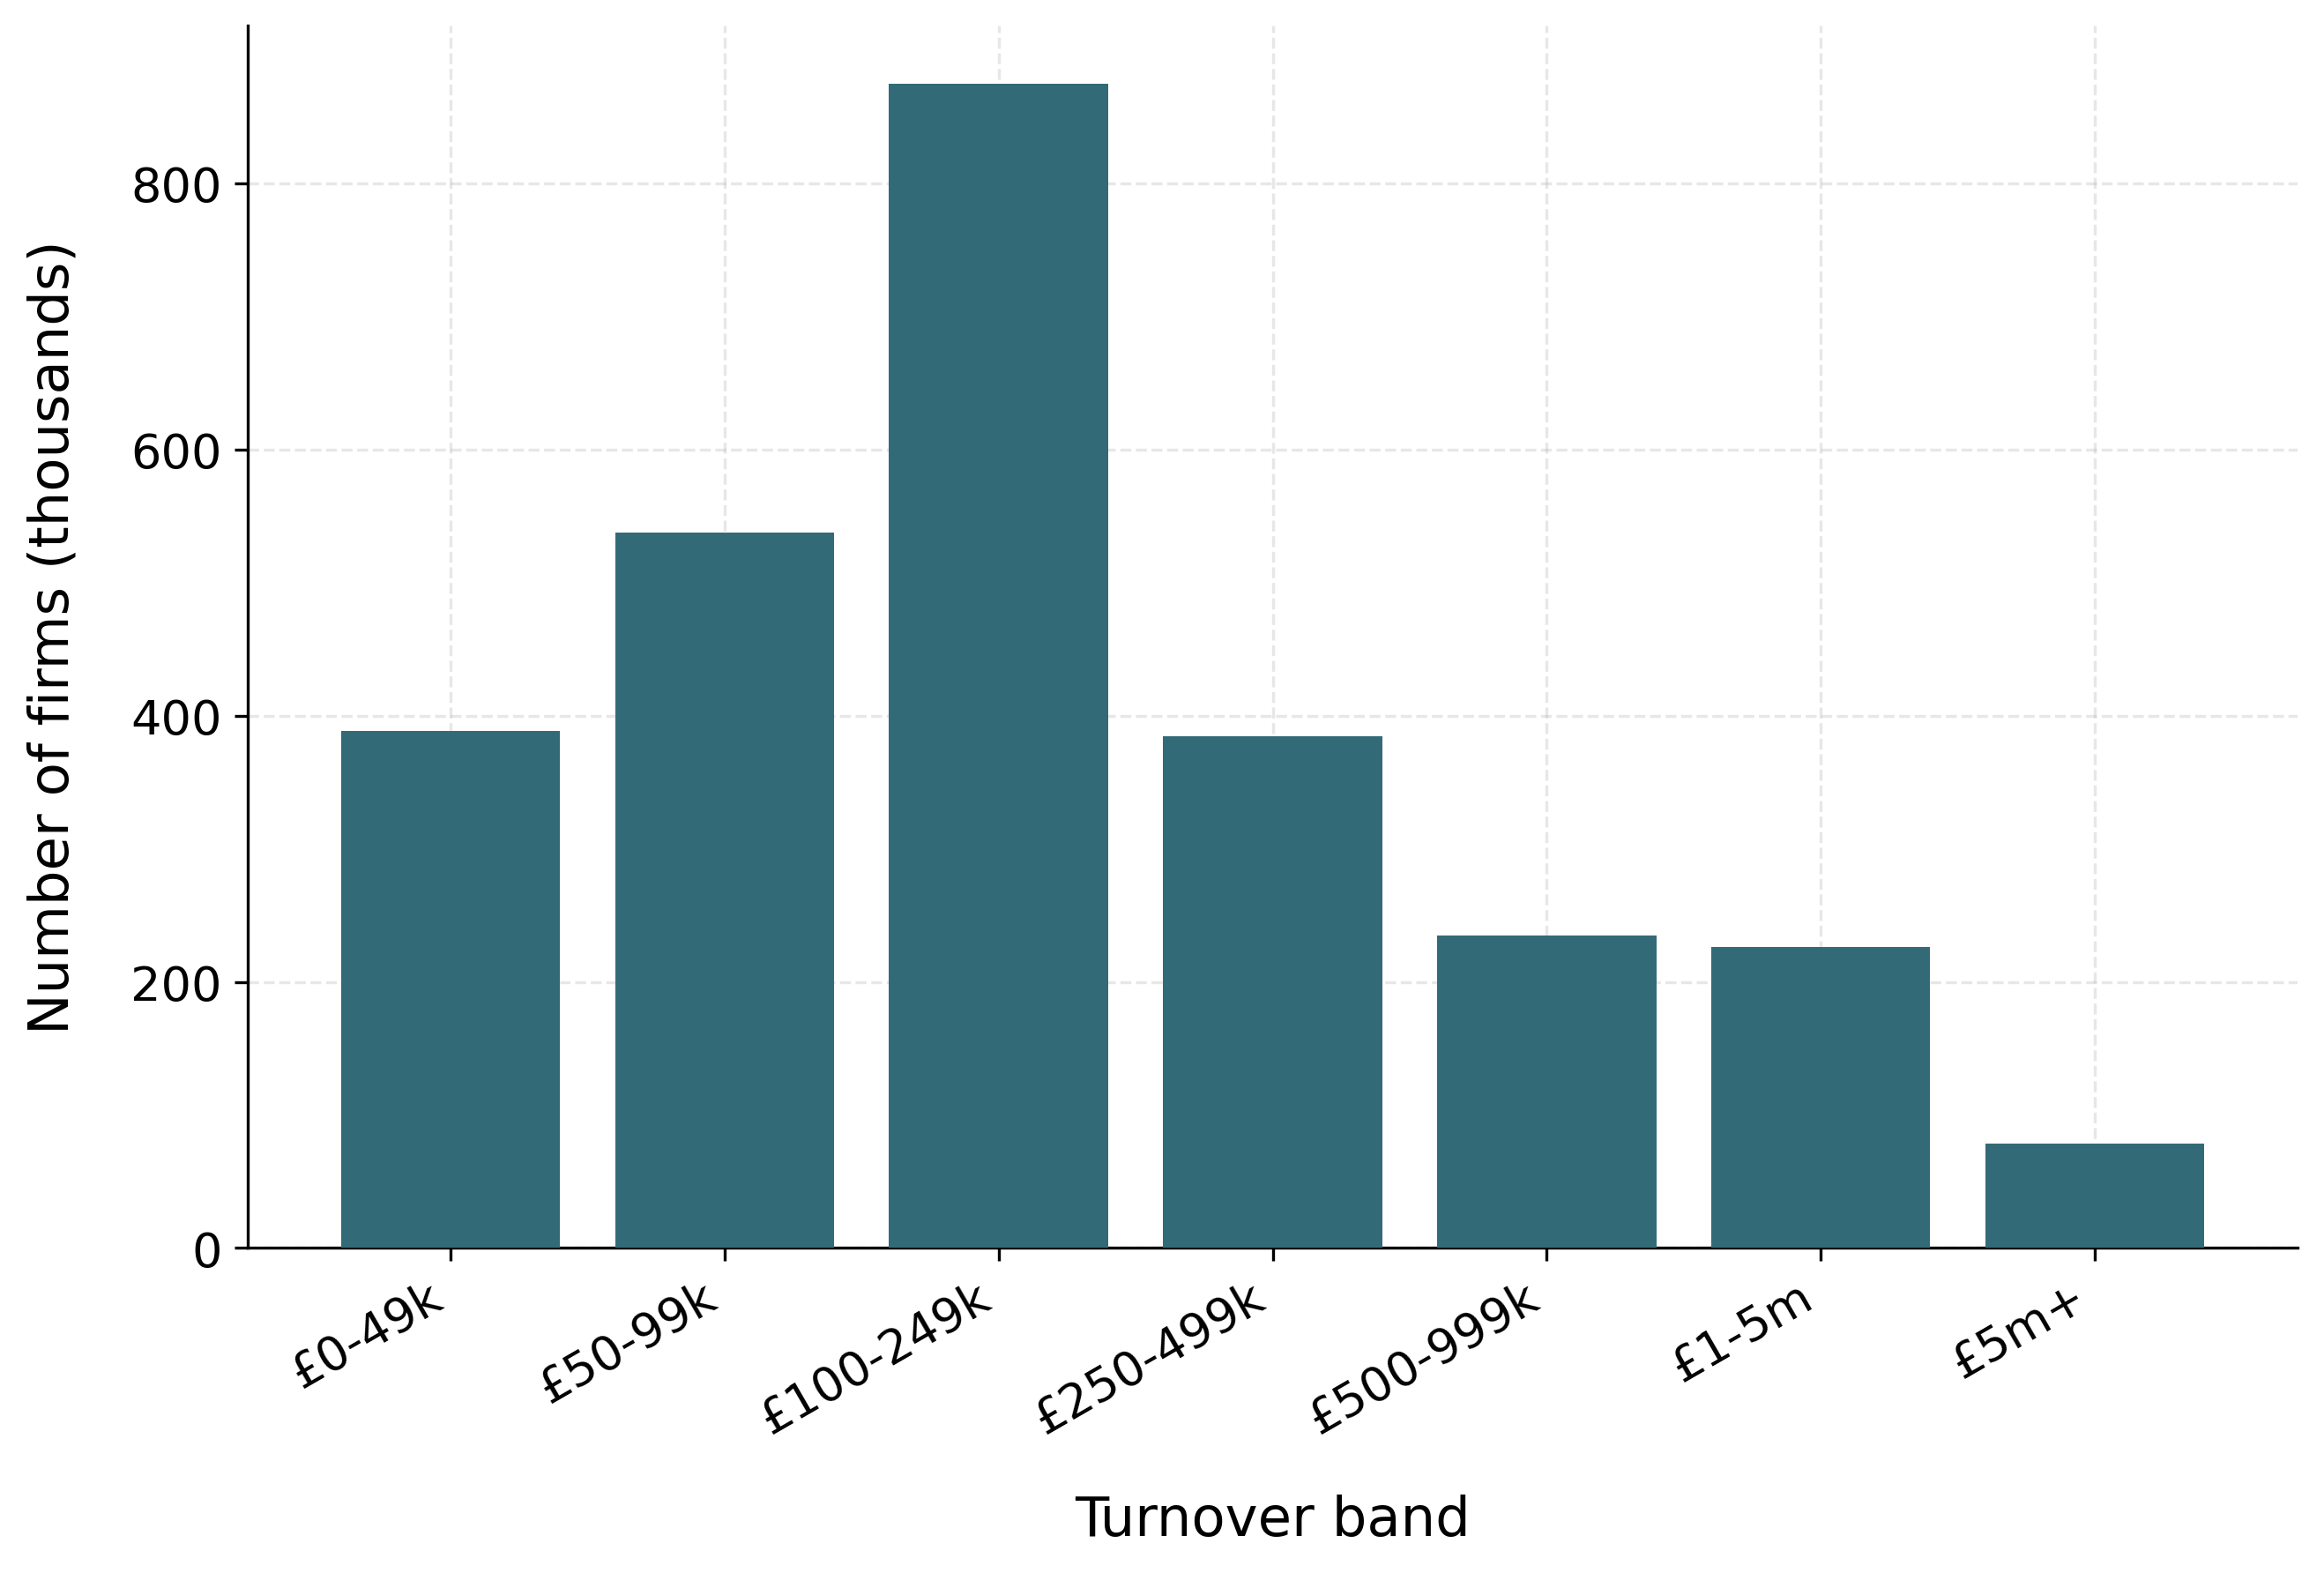
\includegraphics[width=0.98\colwidth]{figures/firms_by_turnover_band_85k.png}
  \end{figure}

  \begin{block}{Three reform families, one basis}
    Costed on a \emph{common static basis}:
    \begin{itemize}
      \item \hl{Level} --- move the threshold up or down.
      \item \hl{Shape} --- a graduated taper that phases VAT in.
      \item \hl{Rate} --- a reduced-rate band above the threshold.
    \end{itemize}
  \end{block}

  \begin{alertblock}{Contribution}
    An open, reproducible firm-level microsimulation that:
    \begin{enumerate}
      \item costs \hl{level + shape + rate} reforms on one static basis;
      \item characterises the notch's distortion via its exact,
            \hl{elasticity-free dominated region};
      \item shows via a \hl{placebo} that synthetic bunching is mechanical;
      \item adds a conditional \hl{behavioural layer}.
    \end{enumerate}
  \end{alertblock}

  \begin{figure}
    \centering
    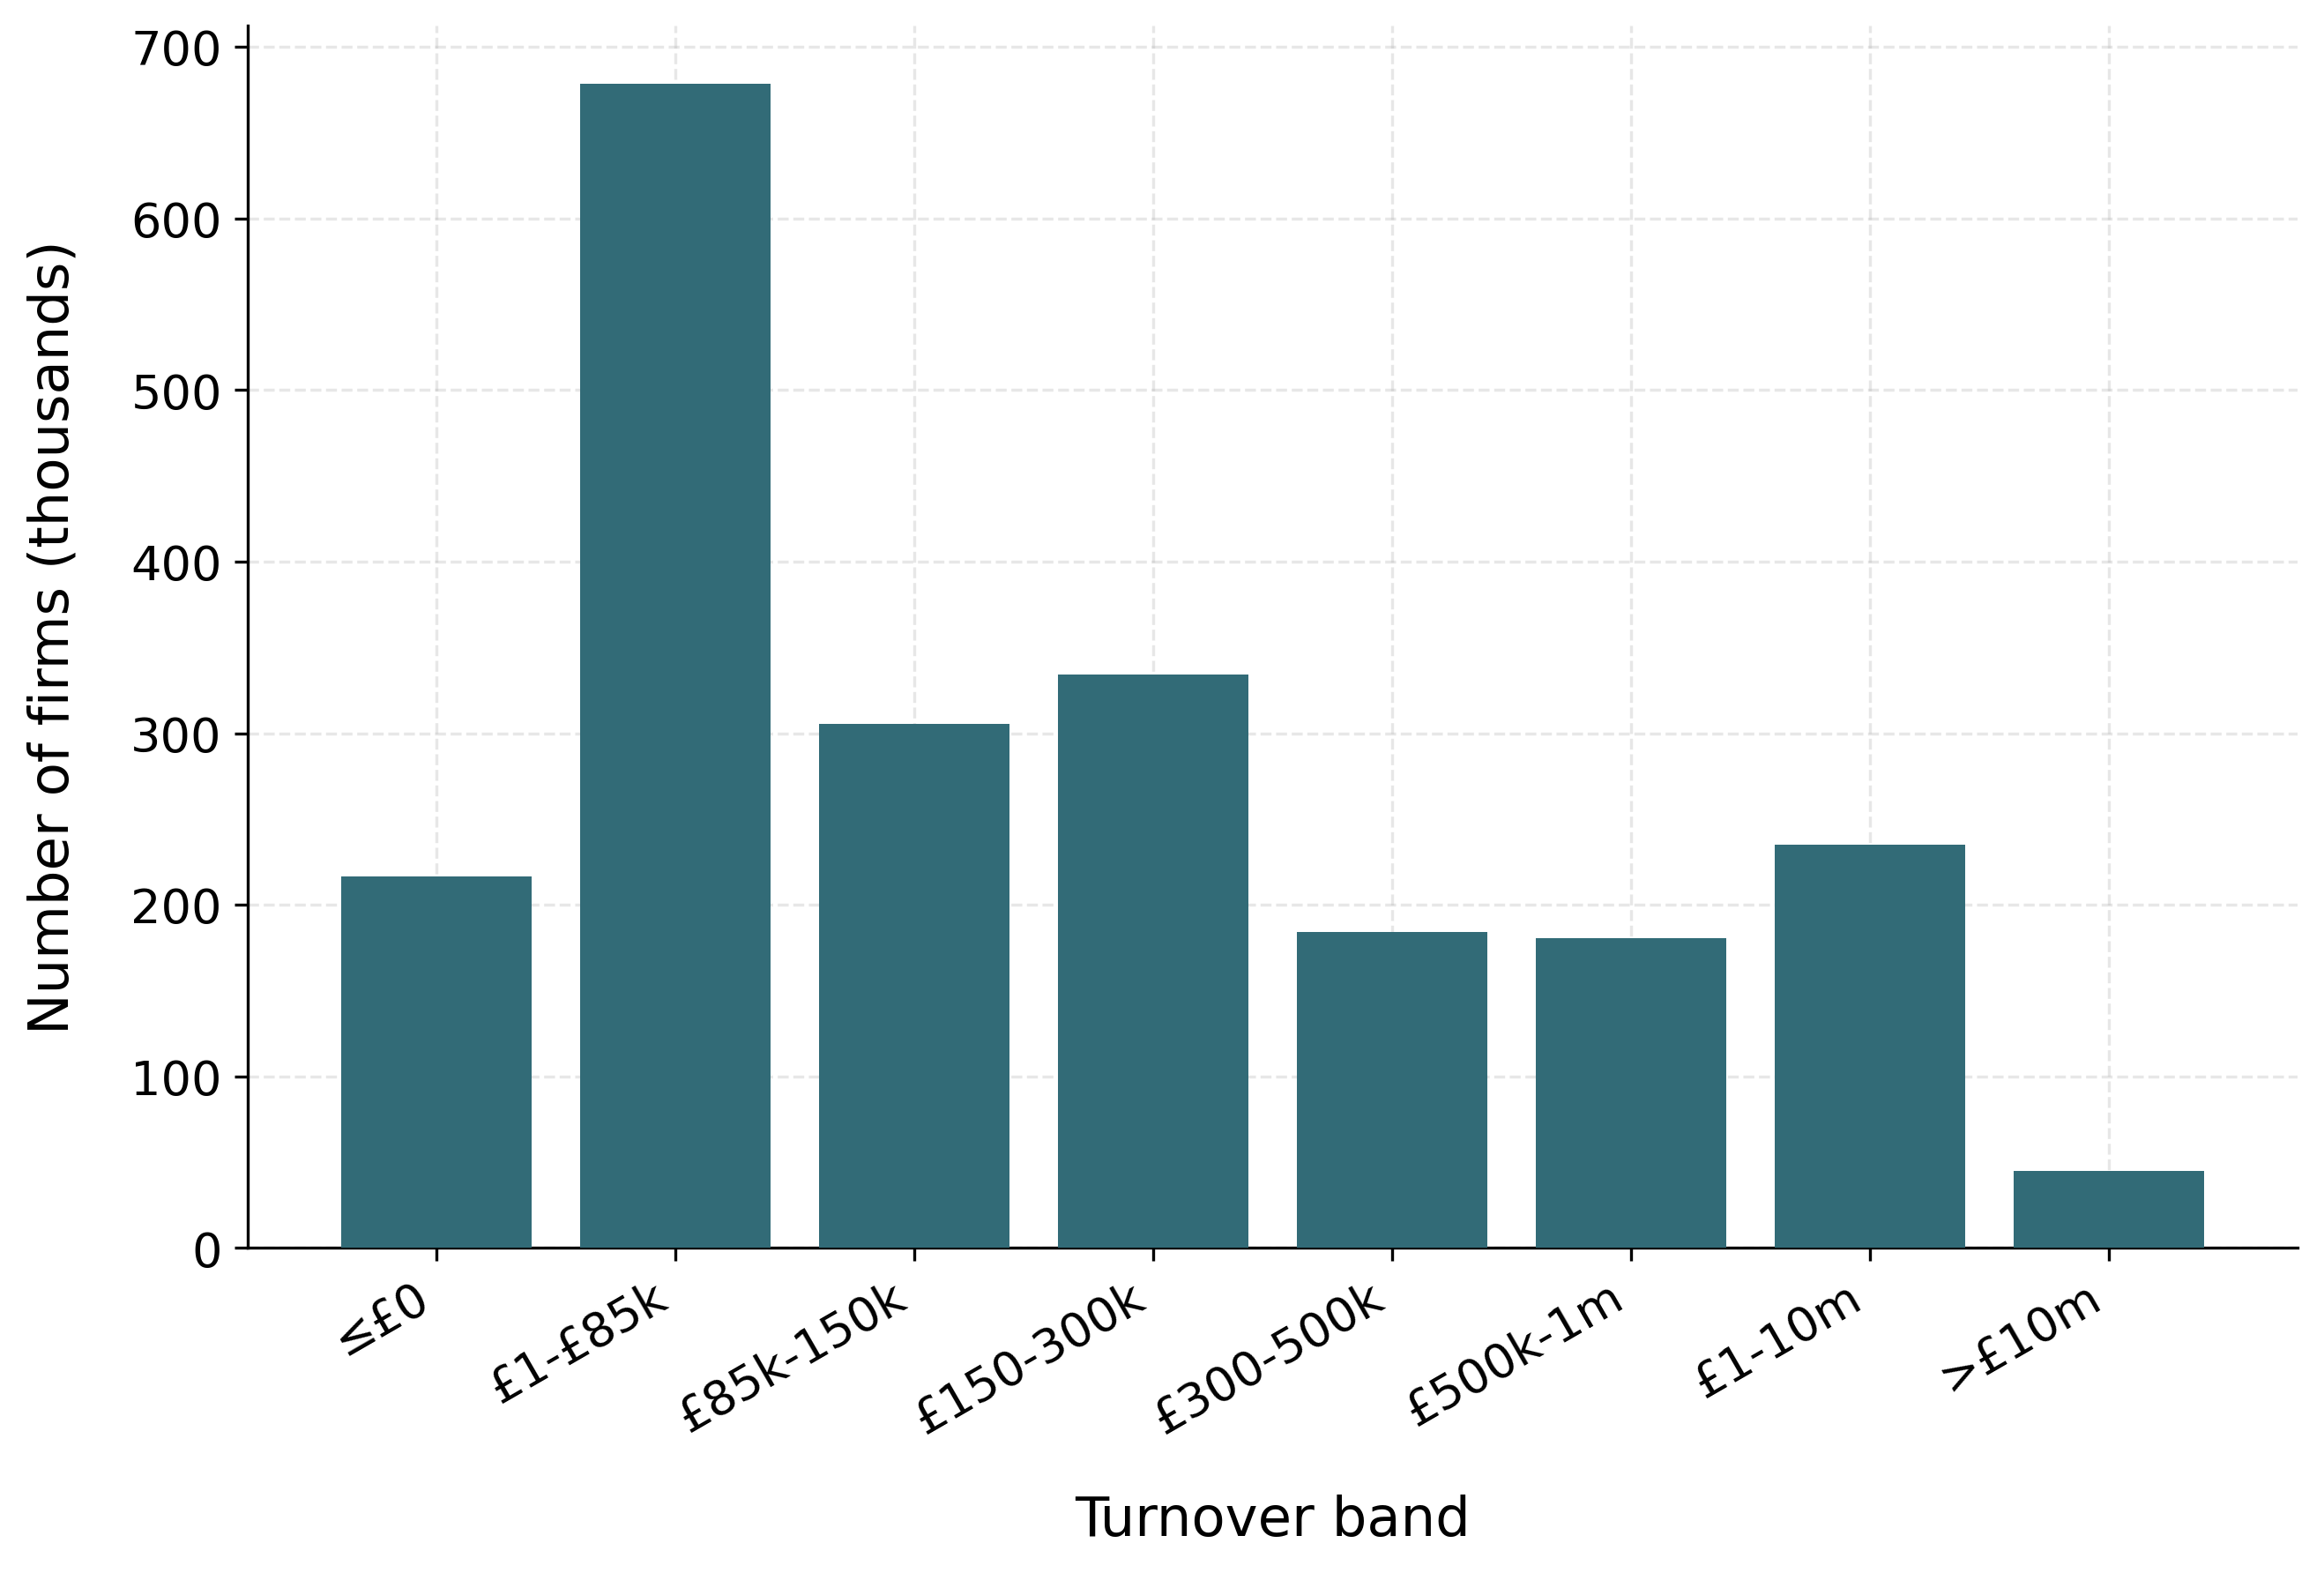
\includegraphics[width=0.84\colwidth]{figures/vat_firms_by_turnover_band_85k.png}
  \end{figure}

  \begin{exampleblock}{Method in one line}
    Draw synthetic firms by sector\,$\times$\,turnover band; assign value
    added $v_i=y_i-x_i$. The threshold is a \emph{generator parameter}, so
    data regenerate under any counterfactual. Firm weights $w_i=e^{\theta_i}$
    are fit by gradient descent to HMRC + ONS aggregates.
  \end{exampleblock}

\end{column}

\separatorcolumn

% ============================== COLUMN 2 ==============================
\begin{column}{\colwidth}

  \begin{block}{Synthetic firm data}
    \hl{$\approx$2.94m} firm rows weighted to \hl{$\approx$2.5m} UK firms,
    calibrated to HMRC + ONS aggregates (turnover-band counts, sector,
    employment, net VAT liability by band) at \hl{$\approx$90\% accuracy}.
    Calibrated \emph{to} the aggregates, so agreement is an
    \hl{internal-consistency check}, not external validation.
  \end{block}

  \begin{figure}
    \centering
    
\includegraphics[width=0.98\colwidth]{figures/turnover_distribution_85k.png}
  \end{figure}

  \begin{exampleblock}{Static costing}
    \[ R(T)=\sum_i w_i\, v_i\,\mathds{1}\{y_i\ge T\} \]
    Revenue moves only through firms whose registration status flips.\\[0.4em]
    \hl{Validation vs HMRC:} the \pounds85k$\to$\pounds90k April-2024 increase
    costs \hl{$-$\pounds175m} in 2025--26 vs HMRC's published
    \hl{$-$\pounds185m} --- agreement \hl{within $\sim$\pounds10m}.
  \end{exampleblock}

  \begin{figure}
    \centering
    
\includegraphics[width=0.98\colwidth]{figures/vat_threshold_revenue_impact.png}
  \end{figure}

  \begin{block}{Threshold sweep (2025--26)}
    From a \pounds90k base (\hl{\pounds203.8bn}), the relationship is roughly
    \hl{linear}, $\approx$\pounds150--220m per \pounds5k step.
    \begin{figure}
      \centering
      
\includegraphics[width=0.71\colwidth]{figures/revenue_impact_2025_26.png}
    \end{figure}
  \end{block}

\end{column}

\separatorcolumn

% ============================== COLUMN 3 ==============================
\begin{column}{\colwidth}

  \begin{alertblock}{The dominated region}
    Profit jumps \emph{down} by $\tau T^\ast=\pounds17{,}000$ at the
    threshold. The \hl{dominated region} --- turnover where no firm locates
    because it earns less than at $T^\ast$ --- has exact width
    \[ a=T^\ast\tfrac{\tau}{1-\tau}=\pounds21{,}250 \]
    (\pounds85{,}000--\pounds106{,}250), spanning \hl{$\approx$137{,}000}
    weighted firms. \hl{Exact and elasticity-free} (conditional on the
    turnover-tax notch).
  \end{alertblock}

  \begin{figure}
    \centering
    
\includegraphics[width=0.98\colwidth]{figures/dynamic_notch_fit_e017.png}
  \end{figure}

  \begin{block}{How reforms change it}
    \begin{itemize}
      \item Raising the threshold \hl{relocates} the \pounds21{,}250 band
            unchanged.
      \item A banded reduced rate does \hl{not shrink} it: reverting to 20\%
            at the band top adds a \emph{secondary} notch
            $a'=T_1\tfrac{\tau-r}{1-\tau}$, so total width is
            \hl{\pounds21{,}562 (15\%)} / \hl{\pounds22{,}569 (10\%)} --- it
            \hl{splits} the band, not shrinks it.
      \item \hl{Only the graduated taper removes the distortion} entirely.
    \end{itemize}
  \end{block}

  \begin{exampleblock}{Value-added robustness}
    $\approx$42\% of near-threshold firms are net input creditors /
    near-zero remitters (no notch --- consistent with $\approx$43\%
    voluntary registration); for the rest the value-added dominated region
    has median $\approx$\pounds18{,}650.
  \end{exampleblock}

  \begin{block}{Bunching is mechanical}
    Estimator: $b=0.060$, excess mass \hl{$E=8{,}712$} firms. A
    \hl{placebo} collapses $E$ to \hl{0--99} when the step is removed from
    the calibration target $\Rightarrow$ bunching is inherited from coarse
    HMRC band targets, \emph{not} firm behaviour. A \hl{recovery test}
    recovers $\approx$90\% of an injected signal --- the estimator is
    specific \emph{and} sensitive; the null is a property of the data.
    \begin{figure}
      \centering
      
\includegraphics[width=0.86\colwidth]{figures/bunching_analysis_85k.png}
    \end{figure}
  \end{block}

\end{column}

\separatorcolumn

% ============================== COLUMN 4 ==============================
\begin{column}{\colwidth}

  \begin{block}{Reform menu (common \pounds85k / \pounds183.6bn base)}
    \centering
    \renewcommand{\arraystretch}{1.2}
    \footnotesize
    \begin{tabular}{@{}>{\raggedright\arraybackslash}p{0.34\colwidth} c r >{\raggedright\arraybackslash}p{0.30\colwidth}@{}}
      \toprule
      \textbf{Reform} & \textbf{Type} & \textbf{Static} & \textbf{Dominated region}\\
      \midrule
      Raise to \pounds100k & Location & $-$\pounds508m & relocates, removes none\\
      Taper \pounds85--105k & Shape & $-$\pounds336m & \pos{removed entirely}\\
      Reduced 10\% & Rate & $-$\pounds343m & splits (2nd notch)\\
      Reduced 15\% & Rate & $-$\pounds171m & splits (2nd notch)\\
      \bottomrule
    \end{tabular}
    \begin{figure}
      \centering
      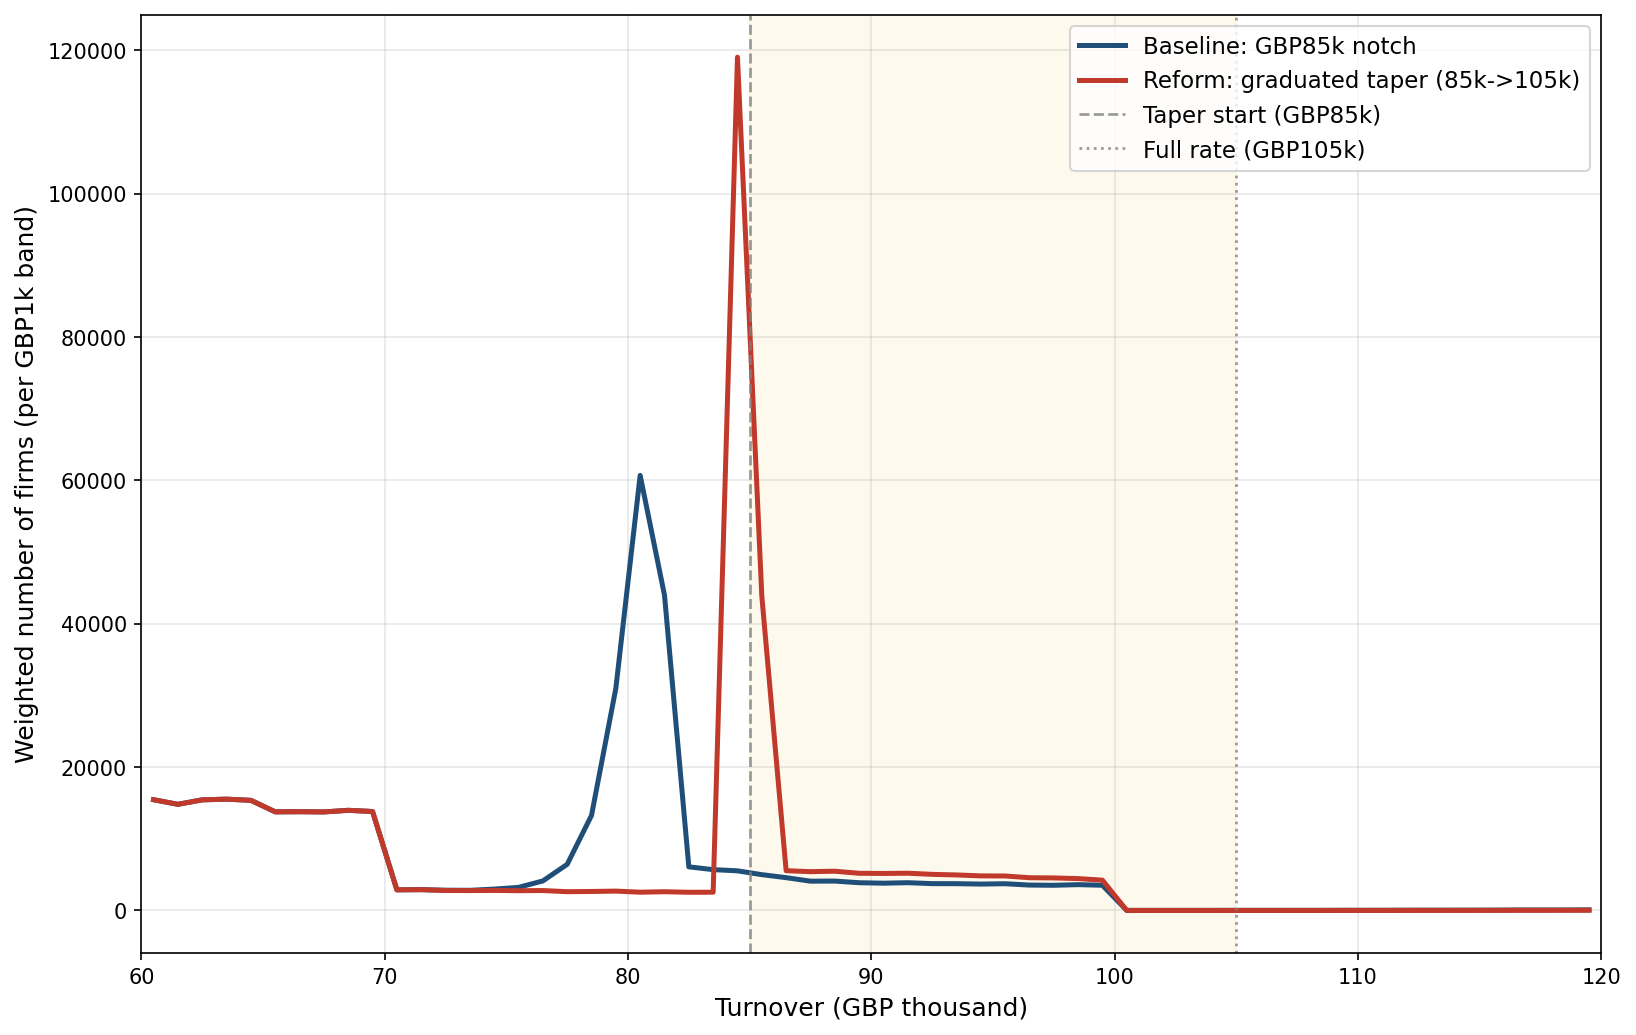
\includegraphics[width=0.80\colwidth]{figures/taper_reform_distribution.png}
    \end{figure}
  \end{block}

  \begin{block}{Behavioural layer (conditional)}
    Conditional on an \hl{assumed} turnover elasticity $e$ (\emph{not}
    identified on synthetic data); sweep $e\in\{0.05,0.17,0.32\}$, midpoint
    $0.17$. At $e=0.17$: raise-to-\pounds100k \pounds508m$\to$\hl{\pounds292m};
    10\% band \pounds343m$\to$\hl{\pounds273m}; 15\% band
    \pounds171m$\to$\hl{\pounds135m}, as firms broaden the base.
    \begin{figure}
      \centering
      
\includegraphics[width=0.72\colwidth]{figures/dynamic_cost_vs_elasticity.png}
    \end{figure}
  \end{block}

  \begin{exampleblock}{Fiscal drag}
    A frozen \pounds90{,}000 threshold draws \hl{$\approx$14\% more firms}
    into the dominated region by 2028--29 ($\approx$130{,}000$\to$148{,}000).
  \end{exampleblock}

  \begin{alertblock}{Conclusions}
    \begin{enumerate}
      \item Prices level + shape + rate on one basis; reproduces HMRC's
            anchor costing.
      \item On the dominated-region metric, \hl{only the taper removes the
            distortion} --- the level move is the dearest and least efficient.
      \item Synthetic bunching is \hl{mechanical} (a transparency lesson) ---
            no elasticity is read off it.
      \item Behavioural offsets are conditional on an assumed $e$; the static
            cost and dominated region are the \hl{elasticity-free anchors}.
    \end{enumerate}
  \end{alertblock}

  \begin{block}{Future work \& contact}
    \begin{minipage}{0.62\colwidth}
      \small Identify $e$ from administrative micro-data; welfare / MVPF
      accounting; sectoral incidence.\\[0.4em]
      \hl{Vahid Ahmadi} --- PolicyEngine\\
      \texttt{github.com/PolicyEngine/}\\\texttt{firm-microsim-paper}
    \end{minipage}\hfill
    \begin{minipage}{0.32\colwidth}
      \centering
      \qrcode[height=3.4cm]{https://github.com/PolicyEngine/firm-microsim-paper}
    \end{minipage}
  \end{block}

\end{column}

\separatorcolumn
\end{columns}
\end{frame}
\end{document}
